\documentclass[11pt]{exam}

\usepackage[utf8]{inputenc}
\usepackage{hyperref}
\usepackage[spanish]{babel}
\usepackage{listings}
\usepackage{float}
\usepackage[table,xcdraw]{xcolor}
\usepackage{graphicx}

\definecolor{codegreen}{rgb}{0,0.6,0}
\definecolor{codegray}{rgb}{0.5,0.5,0.5}
\definecolor{codepurple}{rgb}{0.58,0,0.82}
\definecolor{backcolour}{rgb}{0.95,0.95,0.92}

\lstdefinestyle{mystyle}{
	backgroundcolor=\color{backcolour},   
	commentstyle=\color{codegreen},
	keywordstyle=\color{magenta},
	%numberstyle=\tiny\color{codegray},
	stringstyle=\color{codepurple},
	basicstyle=\ttfamily\footnotesize,
	breakatwhitespace=false,         
	breaklines=true,                 
	captionpos=b,                    
	keepspaces=true,                 
	%numbers=left,                    
	%numbersep=5pt,                  
	showspaces=false,                
	showstringspaces=false,
	showtabs=false,                  
	tabsize=2
}

\lstset{style=mystyle}

\title{Práctica 2}
\author{Laura Rodríguez Navas \\ rodrigueznavas@posgrado.uimp.es}
\date{{\selectlanguage{spanish}\today} }

\pagestyle{plain}

\begin{document}
	
\maketitle

\section{Introducción}\label{introduccion}

{\setlength{\parindent}{0cm}
Esta práctica se apoya en una plataforma que recrea el videojuego clásico \href{1https://en.wikipedia.org/wiki/Pac-Man}{Pac-Man}. Utiliza una versión muy simplificada del juego para poder desarrollar un sistema de control automático y explorar algunas capacidades del Aprendizaje por Refuerzo aprendidas durante la asignatura. Especialmente, en esta práctica se aplica el algoritmo \textit{Q-learning} para construir un agente que funcione de forma automática en los tres mapas disponibles: \textit{lab1.lay, lab2.lay y lab3.lay}. El objetivo de este agente será maximizar la puntuación obtenida en una partida.
}

Asimismo, en este documento se describen las tareas realizadas, que se dividen en distintas fases (definición de los estados, función de refuerzo, construcción del agente y evaluación), y que se detallan a continuación.

En la sección~\ref{estados} se justifica el conjunto de atributos elegido y su rango para la definición de los estados. Una vez se ha elegido el conjunto de atributos que se van a utilizar para representar cada estado, en la sección~\ref{refuerzo} se detalla el diseño de la función de refuerzo que vamos a emplear y que permitirá al agente lograr su objetivo de maximizar la puntuación obtenida en una partida. Después de esto, en la sección~\ref{codigo} se explica cómo se ha procedido a la construcción del agente con el fin de funcionar bien en todos los laberintos. Cuando se obtiene el agente, en la sección~\ref{resultados} se presentan los resultados de las puntuaciones que ha obtenido en los mapas proporcionados y se añaden comentarios sobre su comportamiento. Finalmente, en la parte final del documento se añaden las conclusiones (sección~\ref{conclusiones}) y un apéndice que contiene métodos auxiliares del código desarrollado en las secciones~\ref{refuerzo} y \ref{codigo}.

%\begin{figure}[!htb]
%	\minipage{0.32\textwidth}
%	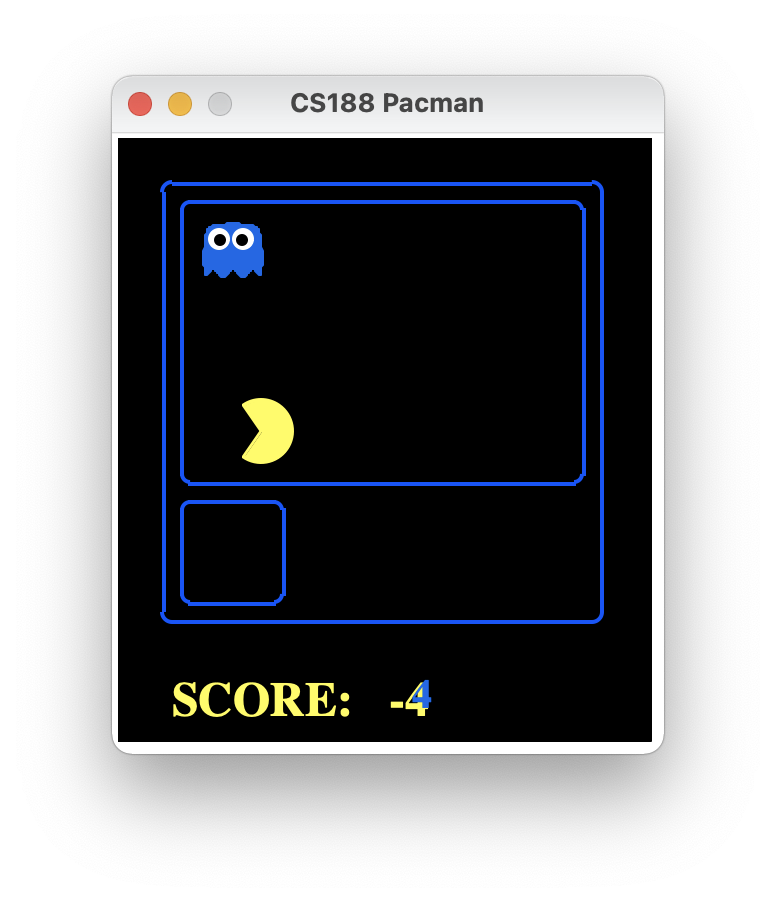
\includegraphics[width=\linewidth]{figures/lab1}
%	\caption{A really Awesome Image}\label{fig:awesome_image1}
%	\endminipage\hfill
%	\minipage{0.32\textwidth}
%	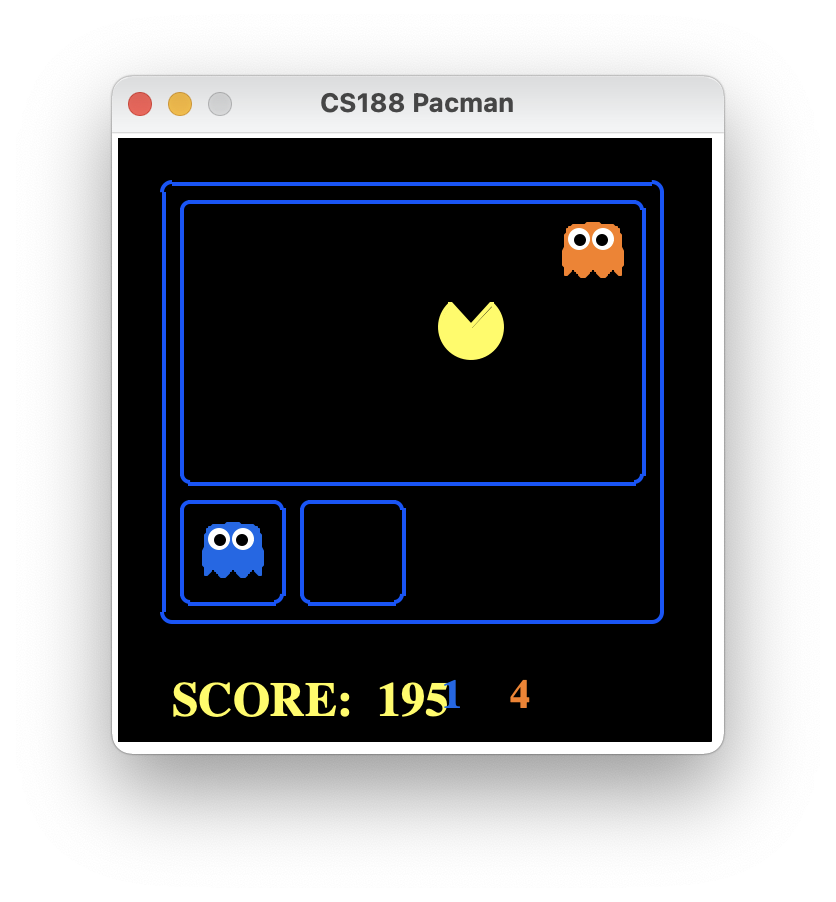
\includegraphics[width=\linewidth]{figures/lab2}
%	\caption{A really Awesome Image}\label{fig:awesome_image2}
%	\endminipage\hfill
%	\minipage{0.32\textwidth}%
%	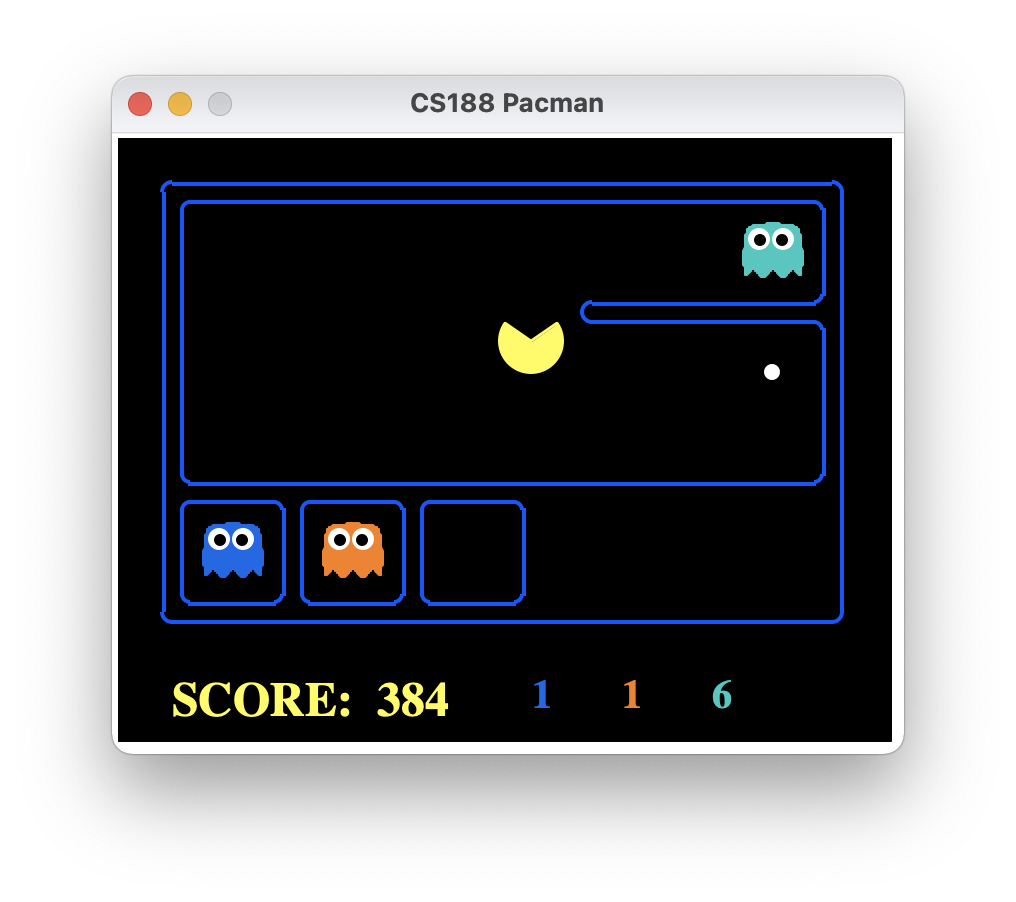
\includegraphics[width=\linewidth]{figures/lab3}
%	\caption{A really Awesome Image}\label{fig:awesome_image3}
%	\endminipage
%\end{figure}

\section{Definición de los estados}\label{estados}

\begin{lstlisting}[language=python, basicstyle=\footnotesize]
self.nRowsQTable = 16
self.alpha = float(0.4)
self.gamma = float(0.9)
self.epsilon = float(1)
self.actions = {"North": 0, "East": 1, "South": 2, "West": 3, "Stop": 4}	
\end{lstlisting}



\section{Función de refuerzo}\label{refuerzo}

\begin{lstlisting}[language=python, basicstyle=\footnotesize]
def getReward(self, state, nextState):
	"""
	Return a reward value based on the information of state and nextState
	"""	
	reward = 0
	
	if nextState.isWin():
	return 1000
	
	next_state_ghost_index_distances = self.getLivingGhostIndexDistances(nextState)
	actual_state_ghost_index_distances = self.getLivingGhostIndexDistances(nextState)
	min_distance_ghost_index_next_State = self.getMinIndex(next_state_ghost_index_distances)[0]
	min_distance_ghost_index_actual_State = self.getMinIndex(actual_state_ghost_index_distances)[0]
	
	min_ghost_distance_next_state = nextState.data.ghostDistances[min_distance_ghost_index_next_State]
	min_ghost_distances_actual_state = state.data.ghostDistances[min_distance_ghost_index_actual_State]
	number_ghost_actual_state = len(self.getAliveGhostDistances(state.data.ghostDistances))
	number_ghost_next_state = len(self.getAliveGhostDistances(nextState.data.ghostDistances))
	actual_state_has_walls = self.directionIsBlocked(state, state.getGhostPositions()[min_distance_ghost_index_next_State])
	next_state_has_walls = self.directionIsBlocked(nextState, nextState.getGhostPositions()[min_distance_ghost_index_next_State])
	
	if number_ghost_next_state < number_ghost_actual_state:
	reward += 100
	
	if min_ghost_distance_next_state < min_ghost_distances_actual_state and not actual_state_has_walls \
	and number_ghost_next_state == number_ghost_actual_state:
	reward += 3
	
	elif min_ghost_distance_next_state > min_ghost_distances_actual_state and actual_state_has_walls \
	and number_ghost_next_state == number_ghost_actual_state:
	reward += 1
	
	elif min_ghost_distance_next_state < min_ghost_distances_actual_state and actual_state_has_walls \
	and number_ghost_next_state == number_ghost_actual_state:
	reward += -1
	
	elif (min_ghost_distance_next_state > min_ghost_distances_actual_state and not actual_state_has_walls) or \
	(min_ghost_distance_next_state == min_ghost_distances_actual_state and number_ghost_next_state == number_ghost_actual_state):
	reward += -min_ghost_distance_next_state
	
	# If next_state_has_walls
	if not actual_state_has_walls and next_state_has_walls and number_ghost_next_state == number_ghost_actual_state:
	reward -= 4
	elif actual_state_has_walls and not next_state_has_walls and number_ghost_next_state == number_ghost_actual_state:
	reward += 1
	
	return reward
\end{lstlisting}


\section{Código desarrollado}\label{codigo}

\begin{lstlisting}[language=python, basicstyle=\footnotesize]
def update(self, state, action, nextState, reward):
	"""
	The parent class calls this to observe a
	state = action => nextState and reward transition.
	You should do your Q-Value update here
	"""
	reward = reward + self.getReward(state, nextState)  # Calculate reward
	
	print "Started in state:"
	self.printInfo(state)
	print "Took action: ", action
	print "Ended in state:"
	self.printInfo(nextState)
	print "Got reward: ", reward
	print "---------------------------------"	
	
	position = self.computePosition(state)
	action_column = self.actions[action] - 1
	sample = reward + self.gamma * self.getValue(nextState)
	
	if nextState.isWin():   # If a terminal state is reached
		self.writeQtable()
	
	else:
		self.q_table[position][action_column] = (1 - self.alpha) * self.q_table[position][action_column] + self.alpha * sample
\end{lstlisting}

Este proyecto se divide en varias tareas pequeñas que deben completarse en consecuencia. La primera tarea gira en torno al diseño de Value-Iteration Agent. Este agente puede planificar su acción dado el conocimiento del entorno antes incluso de interactuar con él. Para ello, debemos calcular los valores Q de las acciones que seguirá el agente y elegir la mejor acción que devolverá el valor Q máximo. Después de diseñar el agente de iteración de valor, necesitamos cambiar el valor de descuento, ruido y vida.
recompensa para lograr la mejor política óptima.

La siguiente tarea es escribir código para Q learning agent. Este agente, a diferencia del agente de iteración de valor, necesita interactuar activamente con el entorno para que pueda aprender a través de las experiencias. Necesitamos aproximar la función Q de los pares estado-acción a partir de las muestras de Q (s, a) que observamos durante la interacción con el medio ambiente. Después de una aproximación exitosa, el agente debería poder tomar la mejor acción para lograr el objetivo. Q-learning Pacman debería poder ganar al menos el 80\% del tiempo.

Sin embargo, a medida que intentamos utilizar este agente en diseños más grandes, por ejemplo, el mundo Grid medio
El entrenamiento de PacMan de alguna manera ya no funcionará bien. Para resolver este problema, debemos
optimizar nuestro agente para implementar también un agente Q-learning aproximado que aprenda los pesos de
características de los estados, donde muchos estados pueden compartir las mismas características.

\section{Resultados}\label{resultados}

\section{Conclusiones}\label{conclusiones}

\section{Apéndice}\label{apendice}

\subsection{Métodos de la función \textit{get\_reward}}

\begin{lstlisting}[language=python, basicstyle=\footnotesize]
	
\end{lstlisting}

\subsection{Métodos de la función \textit{update}}

\begin{lstlisting}[language=python, basicstyle=\footnotesize]
	
\end{lstlisting}

\end{document}
